\documentclass[tikz,border=2pt]{standalone}
\usepackage{amsmath,amssymb}
\usepackage{tikz}
\usetikzlibrary{arrows.meta}

\begin{document}
% The sample variance averages the squared deviations from the sample mean (dividing by
% n - 1): the segments show the deviations x_i - xbar for the eight observations.
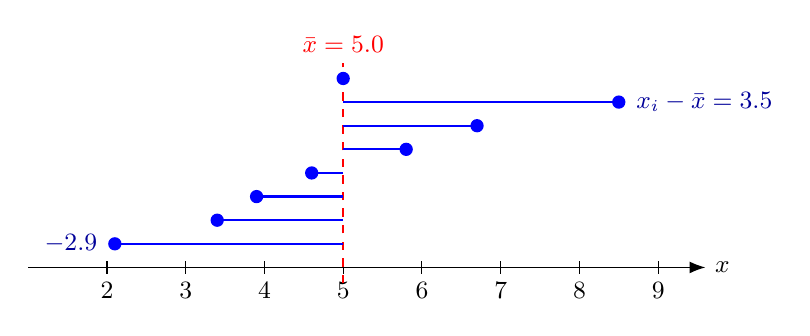
\begin{tikzpicture}[every node/.style={font=\small}, >={Latex[length=2mm]}]
	\draw[->] (1,0) -- (9.6,0) node[right] {$x$};
	\foreach \x in {2,3,...,9} {\draw (\x,0.08) -- (\x,-0.08); \node[below=2pt] at (\x,0) {\x};}
	\draw[red, dashed, thick] (5,-0.2) -- (5,2.6);
	\node[red, anchor=south] at (5,2.6) {$\bar x=5.0$};
	\foreach \x/\y in {2.1/0.3, 3.4/0.6, 3.9/0.9, 4.6/1.2, 5.8/1.5, 6.7/1.8, 8.5/2.1} {
		\draw[blue, thick] (5,\y) -- (\x,\y);
		\fill[blue] (\x,\y) circle (2.4pt);
	}
	\fill[blue] (5.0,2.4) circle (2.4pt);
	\node[blue!60!black, anchor=west] at (8.6,2.1) {$x_i-\bar x=3.5$};
	\node[blue!60!black, anchor=east] at (2.0,0.3) {$-2.9$};
	
\end{tikzpicture}
\end{document}
